%
% File acl2015.tex
%
% Contact: car@ir.hit.edu.cn, gdzhou@suda.edu.cn
%%
%% Based on the style files for ACL-2014, which were, in turn,
%% Based on the style files for ACL-2013, which were, in turn,
%% Based on the style files for ACL-2012, which were, in turn,
%% based on the style files for ACL-2011, which were, in turn,
%% based on the style files for ACL-2010, which were, in turn,
%% based on the style files for ACL-IJCNLP-2009, which were, in turn,
%% based on the style files for EACL-2009 and IJCNLP-2008...

%% Based on the style files for EACL 2006 by
%%e.agirre@ehu.es or Sergi.Balari@uab.es
%% and that of ACL 08 by Joakim Nivre and Noah Smith

\documentclass[11pt]{article}
\usepackage{acl2015}
\usepackage{times}
\usepackage{url}
\usepackage{latexsym}
\usepackage{graphicx}
\usepackage{longtable}
%\setlength\titlebox{5cm}


\title{%
  Scholastic Aptitude of Neural Networks: \\
  \large Improving the performance of word embeddings on analogy questions
}

\author{Felipe Campos \\\And
  Robert Foster \\\And
  Zachary Ingbretsen \\
}

\date{}

\begin{document}
\maketitle
\begin{abstract}
Understanding the relationships between abstract concepts is a valuable skill for both humans and computers. A somewhat surprising property of word embeddings trained by CBOW or skip-gram neural network models is that linear relationships form between words. We are putting word embeddings trained on different corpora to the test. First, we show how the embeddings perform on a standardized set of analogy questions from Turney, et. al. In the future, we will explore methods of improving the performance of a subset of these word embeddings.\end{abstract}

\section{Introduction}

This paper studies different approaches to computationally process
analogies. A good understanding of analogies is crucial for better
understanding the meaning and usage of words in human-written texts and
may be generalizable to other areas of AI development. First, we use
pre-trained word embeddings (Word2vec and GloVe) to establish a baseline
of how word embeddings perform at this problem. We establish performance
differences based on the training corpus, number of dimensions, and
distance metric used. Given that understanding, we attempt to improve on
the performance of the embeddings by analyzing their shortcomings and
augmenting them. Specifically, we use ELMo representations of our words
to improve on the GloVe embeddings, and we train a deep neural net on
analogy questions.

\section{Background}

The analogy task from Turney, et. al. has been subjected to various
approaches since the early 2000's. There are many approaches that exceed
the baseline performance of random guessing, however no automated
approaches excel at this task. Somewhat consolingly, humans also do not
excel at the task; The average US college applicant only scores a 57\%
on this particular test (Turney and Littman, 2005). The current state of
the art on this task is a hybrid ConceptNet implementation which scores
a 56.1\%, approaching the performance of the average college
applicant(Speer et. al., 2017).

\subsection{Challenges}

Understanding analogies requires identifying the correct meaning of
individual words and the relationships between pairs of words. Correctly
answering a seemingly simple analogy could involve first disambiguating
homonyms, and then identifying complex/non-linear relationships between
words, among other challenges. Our work tries to address the following
problems.

\subsection{One-to-Many Relationships}

A relationship such as capital-to-country has a straightforward
interpretation. Italy has only one capital, and that capital is Rome.
Such a one-to-one relationship can be applied to all countries in order
to find the capital. However, there is no such relationship between any
arbitrary city and its country. Naples is a city in Italy, but the
city's relationship in high-dimensional space does not occupy a
privileged position, as does the capital city. For this reason, a linear
transformation may not be effective at correctly answering this type of
analogy. One solution idea to this problem was to use a web search to
find the words (Bollegala et. al., 2008). Overall this was only
moderately effective

\subsection{Polysemy}

Having just one embedding per word can be problematic if a word has more
than one meaning. Over the course of training the embedding, all
meanings of the word will contribute to the final embedding. This will
reduce the usefulness of the embedding for all senses of the word.

\subsection{Out of Vocabulary Words}

Word2vec and GloVe are both trained on a large corpus, and filter out
words that do not pass a certain count threshold. If a word in the test
set was not found in the original corpus or did not surpass the count
threshold, it will be impossible to predict an embedding vector for that
word.

\section{Methods}

Given the challenges inherent in this task, we first benchmarked the
performance of pre-trained Word2vec and GloVe vectors. In order to get a
direct comparison of Word2vec and GloVe on this task, we then trained
our own embeddings on a full dump of English Wikipedia. We used these
benchmarks to identify strong and weak aspects of the different
embeddings.

Using this knowledge, we set out to improve our performance by modifying
the embeddings via ELMo, as well as trying to train a neural network to
use the word embeddings to capture non-linear relationships in the
analogies. By modifying the word embedding vectors to introduce
different representations for individual words via a process such as
generating CoVe embeddings or ELMo representations, we believe that we
can rival the performance of a human agent (ELMo CITE \#TODO). ( \#TODO MOVE UP McCann, et. al., 2017)

\subsection{Embedding Evaluation}

As noted by Mikolov et. al., word embeddings can encode relational similarities
in their vector representations and, when well-trained, analogies in the form
"\emph{king }is to \emph{man }as \emph{queen }is to ..." can be answered with
very simple arithmetics. Therefore, in a word analogy of form a:b::c:d, where
(a,b,c,d) are words, it is expected that the vector resulting from the operation
d - c would share some similarity with the vector resulting from b - a.
Therefore, we could answer an analogy question such as a:b::c:? by calculating:

%% \includegraphics[width=0.07910in,height=0.19530in]{./ObjectReplacements/Object 2}
%% \includegraphics[width=1.78660in,height=0.20000in]{./ObjectReplacements/Object 4},
for every
%% \includegraphics[width=0.39170in,height=0.19530in]{./ObjectReplacements/Object 6}

Where \emph{sim }can be any similarity function such as cosine, when
other works usually refer to the equation by the name \emph{3CosAdd}
(Levy and Goldberg, 2014) or Euclidean. In this paper, we use both
similarity functions for experimentation purposes.

We also evaluate the performance of word embeddings when used in a
neural network trained and focused on solving analogy questions, based
on a deep neural network model used for visual analogy-making in a
previous work (Reed et. al., 2015).

\subsection{Datasets}

An evaluation dataset of 373 SAT questions was obtained from Peter
Turney. Each analogy question has four or five choices as well as part
of speech tagging. We start with benchmarks for the dataset as a whole,
but looked at accuracies for part of speech and question source as well,
using the algorithms below.

Common pre-trained word embeddings (GloVe 6B, 42B, and 840B, and Google
News word2vec) were downloaded from different sources, and we converted
them into the standard Word2vec format to standardize the model scoring
interface.

For training the analogy-focused neural network models, we have used the
Google Analogy Dataset as a smaller training sample (with approximately
20,000 analogies) and the Bigger Analogy Test Set as a more complete
training sample (with more than 2,000,000 analogy questions). The
trained neural network was then benchmarked against the SAT dataset.

\subsection{Code}

The code is written in Bash and Python scripts and is available at:
%% \href{https://github.com/zingbretsenb/w266_final}{\emph{https://github.com/zingbretsenb/w266\_final}}

Instructions on how to run the setup scripts to use the virtual
environment are contained in the Readme.md file in the github
repository. Please email
%% \href{mailto:zingbretsen@berkeley.edu}{\emph{zingbretsen@berkeley.edu}}
your GitHub username for access to the repository if you do not have
access.

\section{Results }

\subsection{Baseline Algorithms}

We used pre-trained word embeddings (word2vec and GloVe trained on
different sources) as a baseline using both Euclidean and cosine
distance measurements. The summary of the baseline models of each are in
Table 1 below:

\begin{table}[h]
\begin{center}
\begin{tabular}{|l|ccc|}
\hline \bf Embeddings & \bf Dims & \bf Euclidean & \bf Cosine \\ \hline
	\bf Twitter.42B & 200 & 0.2172 & 0.2601 \\
	\bf GloVe.6B & 50 & 0.3190 & 0.3566 \\
	\bf GloVe.6B & 100 & 0.3432 & 0.3727 \\
	\bf GloVe.6B & 200 & 0.3405 & 0.4075 \\
	\bf GloVe.6B & 300 & 0.3405 & 0.4155 \\
	\bf GloVe.42B & 300 & 0.3780 & 0.4450 \\
	\bf GloVe.840B & 300 & 0.3619 & 0.4906 \\
	\bf Word2vec & 300 & 0.3190 & 0.4236 \\\hline
\end{tabular}
\end{center}
\caption{\label{font-table} Baseline accuracy of embeddings with different distance metrics.}
\end{table}

\begin{table}[h]
\begin{center}
\begin{tabular}{|l|ccc|}
\hline\bf Embedding & \bf Dims & \bf Diff. PoS & \bf Same PoS \\\hline
\bf Twitter.42B & 200 & 0.318 & 0.340 \\
\bf Glove.6B & 50 & 0.356 & 0.366 \\
\bf Glove.6B & 100 & 0.326 & 0.409 \\
\bf Glove.6B & 200 & 0.356 & 0.448 \\
\bf Glove.6B & 300 & 0.370 & 0.453 \\
\bf Glove.42b & 300 & 0.410 & 0.468 \\
\bf Word2vec & 300 & 0.407 & 0.448 \\\hline
\end{tabular}
\end{center}
\caption{\label{font-table} Accuracy of embeddings when the two words in the analogy were the same or different part of speech.}
\end{table}

From this baseline, we decided to do a direct comparison between
corpora, embeddings and distance metrics. Using the GloVe 42B Twitter
Vectors, the Cosine Distance outperformed the Euclidean Distance with a
26\% vs 22\% accuracy. Also GloVe outperformed word2vec by a small
margin - 40.5\% to 37\% accuracy when they were both trained on the
Wikipedia 4.2B word dataset.

We have so far found the best performance from embeddings with higher
dimensionality, trained on more data, and using cosine distance as the
distance metric. However, there may be cases when the Euclidean distance
is more appropriate to use (e.g., when the analogy has more to do with
the magnitude of the difference between words than direction).

We intend to experiment with different ways of modifying the embeddings
to better encode relationships between words as well as try to train our
own analogy-focused word embeddings to see how they compare against the
baseline.

\subsection{Error Discovery}

Next we examined errors from the best performing embeddings, the GloVe.840B, 300
dimension embedding. The model appeared to have more difficulty with a couple of
relationships more often than others. For example, all of the embeddings got a
question wrong where the analogy was sandal:footwear. All models chose
child:parent as the answer, but the answer was watch:timepiece.

A linear relationship does not capture this relationship well. A sandal
is a type of footwear. However, there are many types of footwear, and
all may have different types of linear relationships. The same is true
for the correct answer: a watch is a type of timepiece. We will need a
different approach to capture relationships like this.

We also investigated errors in the difference between a variety of
relationships using the Google analogies dataset published by Mikolov et
al. The results are shown below in Table 3. As noted in the table, most
Semantic Questions are answered correctly fairly accurately (with the
exception of currency) while most Syntactic Questions are answered less
accurately (Table 4).

For these two reasons, we thought that a purely linear approach to
solving the problem was limiting the types of questions the model could
get correct. We decided to try a couple of approaches to see if we could
overcome this hurdle.


\begin{table}[h]
\begin{center}
\begin{tabular}{|l|c|}
\hline\bf Question Type & \bf ACC \\\hline
\bf Capitals of common countries & 94.66\% \\
\bf Capital of the world & 96.26\% \\
\bf Currency & 5.77\% \\
\bf City in state & 64.69\% \\
\bf Family & 78.46\% \\ \hline
\end{tabular}
\end{center}
\caption{\label{font-table} Accuracy of GloVe.840B 300D embeddings on semantic questions.}
\end{table}


\begin{table}[h]
\begin{center}
\begin{tabular}{|l|c|}
\hline\bf Question Type & ACC \\\hline
\bf Adjective to adverb & 29.33\% \\
\bf Opposite & 31.16\% \\
\bf Comparative & 77.33\% \\
\bf Superlative & 38.24\% \\
\bf Present participle & 59.00\% \\
\bf Nationality adjective & 92.50\% \\
\bf Past tense & 48.21\% \\
\bf Plural & 82.28\% \\
\bf Plural verbs & 51.38\% \\\hline
\end{tabular}
\end{center}
\caption{\label{font-table} Accuracy of GloVe.840B 300D embeddings on syntactic questions.}
\end{table}

\subsection{Improving on Baseline}

To solve the analogy problem, we tried a few different solutions. The first was
to train new embeddings that has more context included for the words using the
ELMo embedding algorithm. The second was to train a deep convolutional neural
network to understand the analogies and make better guesses at the answers.

\subsection{ELMo Encoding Algorithm}

The ELMo algorithm is deep contextualized word representation that
models both (1) complex characteristics of word use (e.g., syntax and
semantics), and (2) how these uses vary across linguistic contexts
(Peters et. al. 2018). The ELMo algorithm can be trained on words or
sentences to produce word embeddings that include more context around
each word. ELMo word representations are functions of the entire input
sentence and are computed on top of two-layer bi-directional LSTMs with
character convolutions as a linear function of the internal network
states. (Peters et. al. 2018). Each layer of the ELMo encodings can be
used as the embedding for our problem set which allows multiple end
`outputs' to the algorithm.

For our ELMo testing, we broke down this phase into two separate
training tests: on each analogy word and on each pair of words. The
baseline vectors in ELMo are the GloVe6B 100 dimension set with a
baseline accuracy of 37.27\%. Table 4 contains the accuracy from
different stages.

%% \begin{longtable}[]{@{}lll@{}}
%% \toprule
%% Type & Layer Output & Accuracy\tabularnewline
%% single & layer-0 & 0.364611\tabularnewline
%% single & layer-1 & 0.455764\tabularnewline
%% single & layer-2 & 0.423592\tabularnewline
%% single & layer-all & 0.412869\tabularnewline
%% pairs & layer-0 & 0.364611\tabularnewline
%% pairs & layer-1 & 0.436997\tabularnewline
%% pairs & layer-2 & 0.399464\tabularnewline
%% pairs & layer-all & 0.407507\tabularnewline
%% \bottomrule
%% \end{longtable}

%% \textbf{Table 4: Accuracy per Stage}

From Table 4, the single word embeddings taken from the first layer
provide the biggest increase in accuracy with a total of 8.3\% from the
baseline accuracy.

\subsection{Neural Network}

We also wanted to test the behavior of embeddings when used in a Neural
Network focused on analogy-making, under the rationale that it could
perhaps find patterns between the encoding of words that is not obvious
with simple vector operations. The neural network architecture was
inspired by the paper "Deep Visual Analogy-Making", by Scott Reed et al,
that used a neural network in the context of visual analogies (e.g.
where images were rotated, changed color and/or changed size). This was
done by encoding pictures using a function \emph{f} and decoding using a
function \emph{g}. Using the a:b :: c:d framework for analogies, the
pictures were inferred by the relationship between a and b by
subtracting the encoded values and then used a transformation query
\emph{T} on c to then decode the result and get d. In the paper, they
used three different types of transformation query for \emph{T}:
\emph{3CosAdd} (as we have done previously), \emph{3CosMul} (similar to
\emph{3CosAdd}, but instead of summing the difference of a and b to c a
multiplication is used) and a deep neural network. We used the latter as
inspiration for our neural network model.

We tried to reproduce a similar approach for words. For this, we changed
the encoding function \emph{f} to a word embedding lookup, based on the
different embeddings we used above. We used the similar approach of
inputting a concatenation of the embedding of the word (c) and the
difference between the embeddings for two given words (a: b) into a
fully-connected neural network, and then summed the results with the
word (c) to achieve the final embedding. This embedding was then decoded
back using decoder function \emph{g }to a word (d) by picking the
closest word in the embedding matrix through either cosine similarity or
euclidean distance. The architecture diagram for the neural network is
shown in figure XX.

The neural network was trained using the following objective function,
similar to the one used in the original paper, which aims to reduce the
sum of the square of norms for the vector resulting from the subtraction
of the encoding of target word d and the decoded result as shown below:

\begin{figure}
  \centering
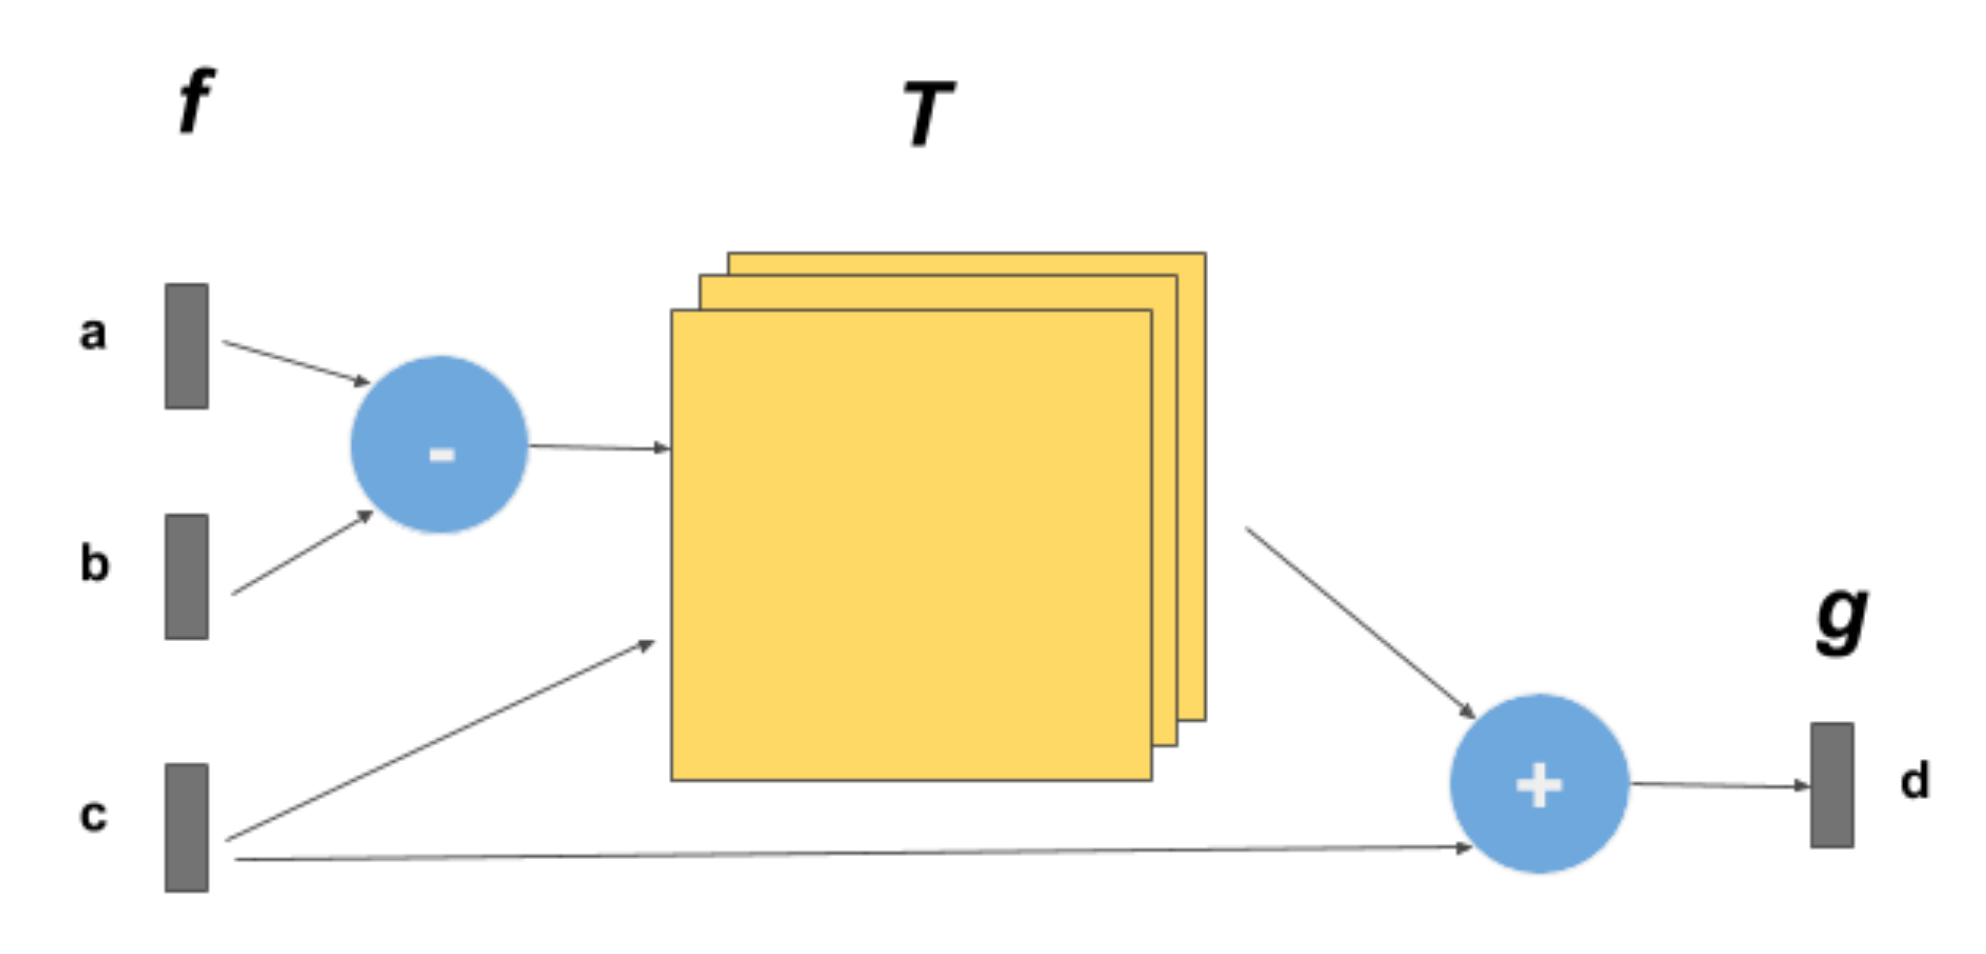
\includegraphics[width=3.0in,height=1.5in]{./model_1.png}
  \caption{Model 1}
\end{figure}

As the original paper did not mention the parameters used for the
fully-connected layers, we have tried with several different network
sizes. Initially, we tried with a single 600-dimensional layer, and then
tried with a bigger model using 4096-2048-1024 dimensional layers.
Training was performed for 4500 epochs with mini-batches of 50 using
Adam Optimizer with gradient clippings with maximum gradient norm of
1.0, learning rate of 0.00001, and with dropout rate of 0.5 using the
Google Analogy dataset. The word embeddings were fixed and made not
trainable in the model, as the interest of our study was to use the
neural network to find word features encoded in the embeddings and not
refine them with analogy data.

After the set amount of epochs, the training still showed room for loss
reduction in case more epochs were executed. The resulting model,
however, failed to produce useful results. It is worth mentioning,
however, that the model did produce word embeddings in the vicinity of
the correct answer in vector space, which indicates that perhaps with some more training epochs to
reduce loss the model could provide better results.

We also developed two other models, which haven't been as thoroughly
tested. In our second model attempt, we tried a modified version by
removing the subtraction between the embeddings of the two given words
(a:b) and inputting a concatenation of all three known words (a:b :: c:)
into the neural network to check whether it would behave better or worse
than the previous model. The rationale was that maybe performing the
subtraction before could be restricting the model to transformations
that are visible in a linear space. The diagram for this architecture is
depicted in figure YY.

\begin{figure}
  \centering
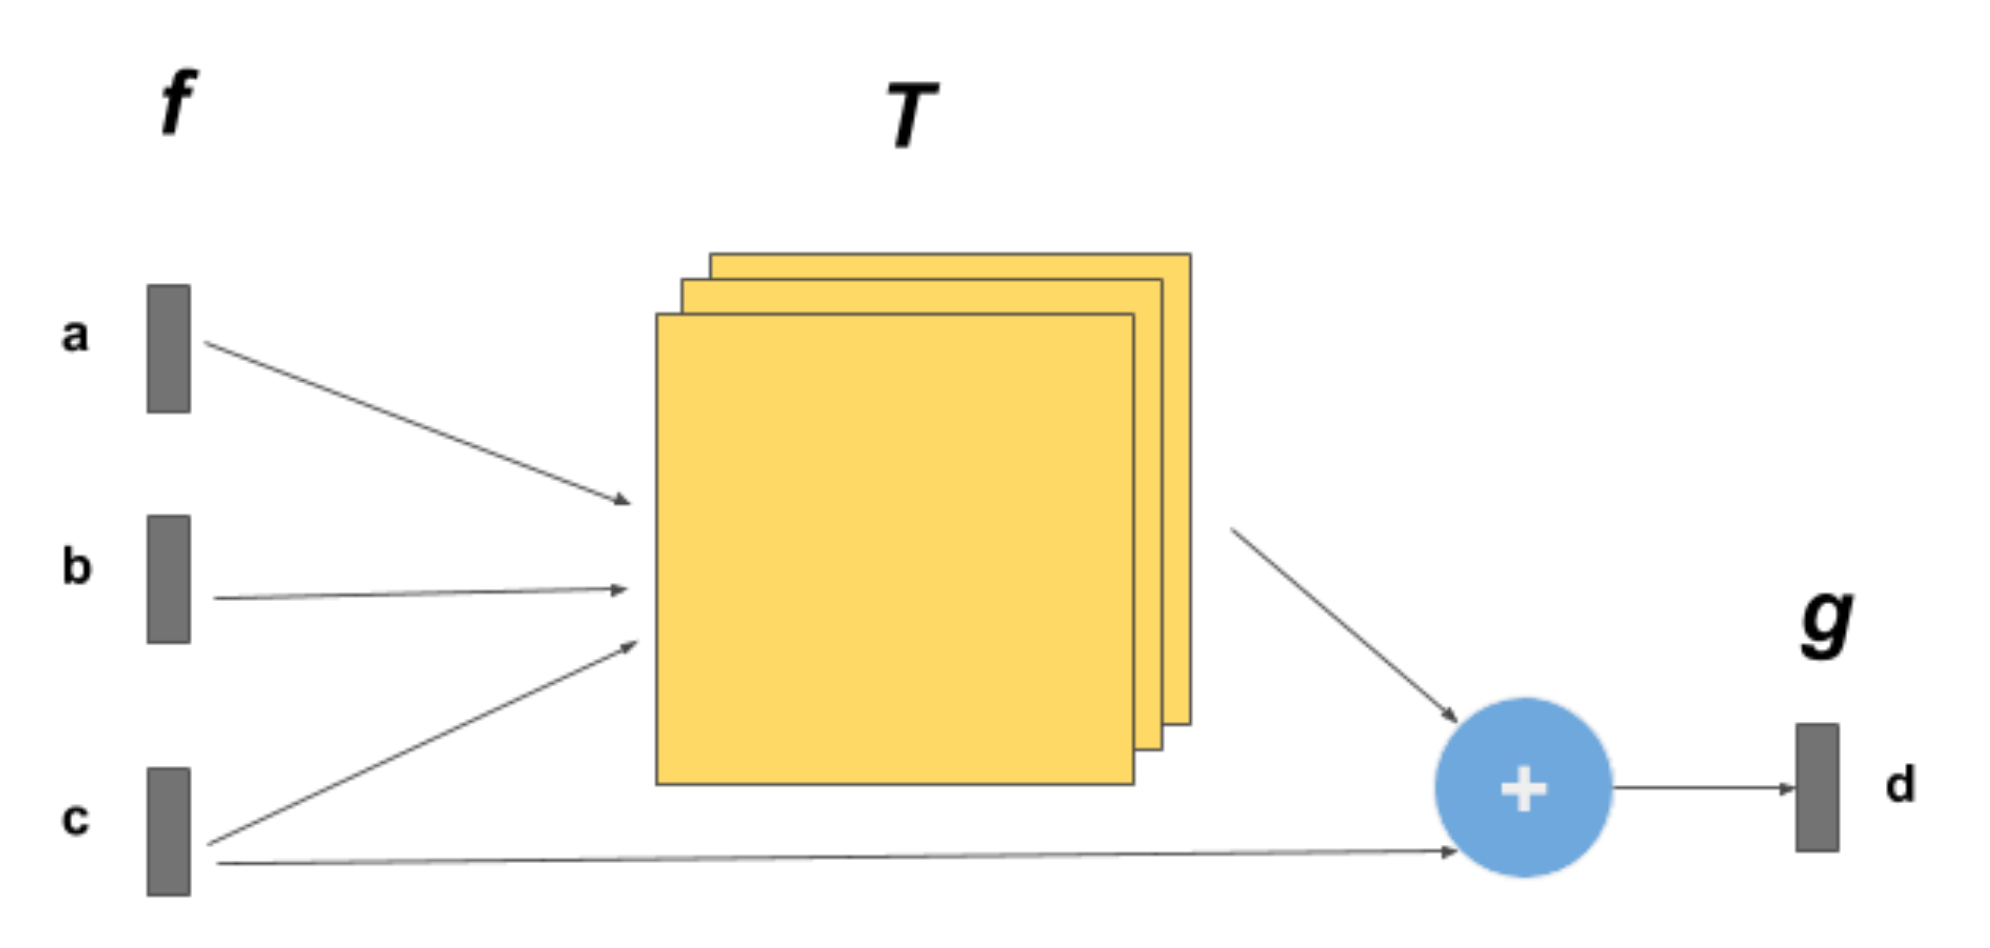
\includegraphics[width=3.0in,height=1.5in]{./model_2.png}
  \caption{Model 2}
\end{figure}

Our third model added a secondary, trainable embedding that is
concatenated with the original, primary embedding through the secondary
encoding function \emph{h}. This aims to augment the original embeddings
with data from training on analogies and perhaps make more complex
analogies clearer on the embedding. The diagram for this architecture is
depicted in figure ZZ. Unfortunately, both models also failed to produce
a noteworthy result that was better than random chance.

\begin{figure}
  \centering
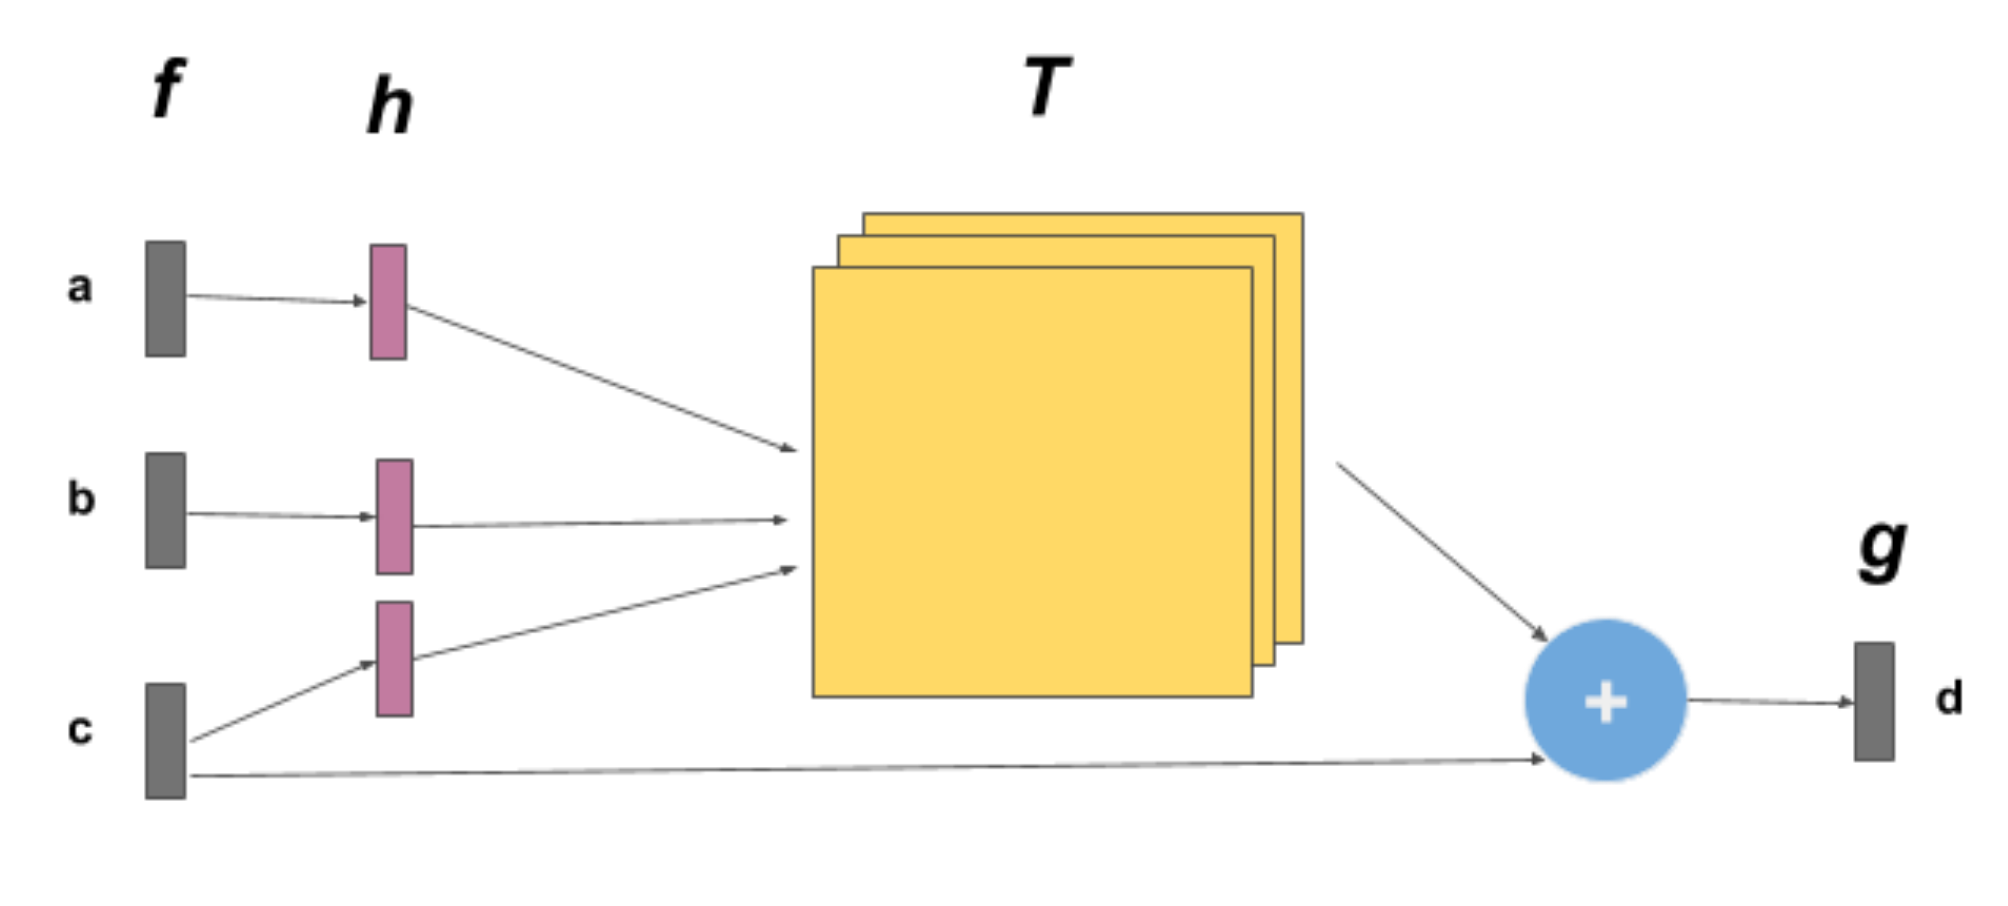
\includegraphics[width=3.0in,height=1.5in]{./model_3.png}
  \caption{Model 3}
\end{figure}

\section{Conclusion}

There are a few lessons to be learned. Unsurprisingly, the quality and
site of the training corpus is important for the performance of word
embeddings on the analogy task, and using the cosine distance as the
distance metric was universally more accurate. Given the results of our
direct comparison of Word2vec and GloVe, we would recommend using GloVe
as the base for future experimentation over Word2vec for this particular
application. However, further improvements can be made on top of the
embeddings alone.

Using ELMo to improve the GloVe embeddings proved to be particularly
promising. The key insight was to use the middle layer of ELMo's deep
net instead of the top layer. Since the lower layers encode more of the
syntactic information, using the middle layer improved performance in
nearly all syntactic questions, and in one semantic type of question.
The ELMo representations did seem to perform poorly on questions
relating to places (i.e., countries or states), but otherwise improved
significantly on the performance of the GloVe 100 dimensional vectors.

The ELMo model that was trained on the Glove 6B 100D emeddings
outperformed even the Glove 42B 300D embeddings. Given that particularly
encouraging result, training an ELMo model on the Glove 840B 300D
vectors would be a promising next step. Given the raw embeddings'
performance on the task, the addition of the ELMo representation could
offer performance that is competitive with the state of the art.

Finally, although the neural network approach ended up not providing
satisfying results, we did find that it does return word embeddings
close to the expected words. Given that there was still margin to reduce
the loss with more training epochs, it is possible that with a larger
analogy dataset for training, more training epochs and further tuning of
the model parameters the neural network model could prove to be a useful
method for solving analogy problems and thus worth the effort of more
study and experimentation.




\begin{thebibliography}{}

\bibitem[\protect\citename{Bollegala, Matsuo, and Ishizuka}2008]{Bollegala, Matsuo, and Ishizuka:2008}
D. Bollegala, Y. Matsuo, M. Ishizuka
\newblock 2008.
\newblock {\em S.A.T. - Measuring Relational Similarity on the Web}
\newblock https://dl.acm.org/citation.cfm?id=1567281.1567356

\bibitem[\protect\citename{Levy and Goldberg}2014]{Levy and Goldberg:2014}
O. Levy and Y. Goldberg.
\newblock 2014.
\newblock {\em Linguistic Regularities in Sparse and Explicit Word Representations}
\newblock http://www.aclweb.org/anthology/W14-1618

\bibitem[\protect\citename{Li, Summers-Stay}2017]{Li and Summers-Stay:2017}
D. Li, D. Summers-Stay
\newblock 2017.
\newblock {\em Dual Embeddings and Metrics for Relational Similarity}
\newblock http://www.aclweb.org/anthology/W17-6924

\bibitem[\protect\citename{McCann, et al.}2017]{McCann, et al.:2017}
B. McCann, J. Bradbury, C. Xiong, R. Socher
\newblock 2017.
\newblock {\em Learned in Translation: Contextualized Word Vectors}
\newblock https://arxiv.org/pdf/1708.00107.pdf

\bibitem[\protect\citename{Mikolov, Chen, Corrado, Dean }2013]{Mikolov and Corrado:13}
T. Mikolov, K. Chen, G. Corrado, J. Dean.
\newblock 2013.
\newblock {\em Efficient Estimation of Word Representations in Vector Space}
\newblock https://arxiv.org/abs/1301.3781v3

\bibitem[\protect\citename{Peters, et al.}2018]{Peters, et al.:2018}
M.~E. Peters, M. Neumann, M. Iyyer, M. Gardener, C. Clark, K. Lee, L. Zettlemoyer
\newblock 2018.
\newblock {\em Deep contextualized word representations}
\newblock https://arxiv.org/pdf/1802.05365.pdf

\bibitem[\protect\citename{Reed, et al.}2015]{Reed, et al.:2015}
S. Reed, Y. Zhang, Y. Zhang, H. Lee
\newblock 2015.
\newblock {\em Deep Visual Analogy-Making}
\newblock http://papers.nips.cc/paper/5845-deep-visual-analogy-making.pdf

\bibitem[\protect\citename{Reed}2017]{Reed:2017}
S. Ruder
\newblock 2017.
\newblock {\em Word Embeddings in 2017: Trends and future direction}
\newblock http://ruder.io/word-embeddings-2017/

\bibitem[\protect\citename{Speer, Chin, Havasi}2016]{Speer, Chin, Havasi:2016}
R. Speer, J. Chin, C. Havasi
\newblock 2016.
\newblock {\em ConceptNet 5.5: An Open Multilingual Graph of General Knowledge}
\newblock https://arxiv.org/abs/1612.03975

\bibitem[\protect\citename{Turney}2008]{Turney:2008}
P.~D. Turney
\newblock 2008.
\newblock {\em A Uniform Approach to Analogies, Synonyms, Antonyms, and Associations}
\newblock https://arxiv.org/pdf/0809.0124.pdf

\bibitem[\protect\citename{Turney}2002]{Turney:2002}
P.~D. Turney
\newblock 2002.
\newblock {\em A Mining the Web for Synonyms: PMI-IR versus LSA on TOEFL}
\newblock https://arxiv.org/ftp/cs/papers/0212/0212033.pdf

\end{thebibliography}

\end{document}
